\chapterx{——~物理世界的统一}\label{chp:00}

物理学的兴起,是从经典力学开始的。在经典力学之前,人类
的文明中虽然已有不少具有物理价值的发现和发明,但是并不存
在一门独立的物理学。因此,我们在学习经典力学的时候,首先
应当了解:为什么经典力学成了物理学的起点?经典力学在整个
物理学中占据着怎样的地位?

爱因斯坦曾经这样来概括牛顿力学的历史地位;“古代希腊
伟大的唯物主义者坚持主张,一切物质事件都应当归结为一系列
的有规律的原子运动,而不允许把任何生物的意志作为独立的原
因。而且无疑笛卡尔曾按他自己的方式重新探索过这一问题。但
是,在当时,它始终不过是一个大胆的奢望,一个哲学学派的成
问题的理想而已。在牛顿之前,还没有什么实际的结果来支持那
种认为物理因果关系有完整链条的信念。”

这句话的意思是,物理学依赖于一种基本的信念:物理世界
存在着完整的因果链条,即自然界是统一的。牛顿力学则是体现
这种信念的第一个成功的范例。

从牛顿力学的创建到现在,已经有三百多年了,物理学已经
大大发展了,远远超过了经典力学原有的水平。但是,就物理学
的最基本的追求和物理学的总目标来说,却一直没有变化。经典
力学时代的追求和目标,可以说时至今日仍然是整个物理学的追
求和目标。这个最基本的追求和目标,就是自然界的统一。的确,
从整个物理学的发展中,可以看到一条鲜明的主线。这就是执着%分页点
地追求宇宙的统一,找寻支配宇宙万物的最基本最统一的规律。

相信存在统一,努力寻求统一,如果仅仅作为一种自然观,
早在古代已经有了。老子的《道德经》中写有:“道生一、一生
二、二生三、三生万物。”这就是中国古代的一种统一观,它完
全可以与爱因斯坦所提及的古希腊的哲学相媲美。不过,无论在
古代中国或古希腊,统一观都只是一种哲学思辨。

牛顿的力学和古代的哲学不同,它不是思辨地坚持统一观,
而是发展了寻找统一的有效的物理方法。牛顿在他的最重要的力
学著作《自然哲学的数学原理》中阐明了他采用的方法。他在前
言中写道;“我奉献这一作品。作为哲学的数学原理,因为哲学
的全部责任似乎在于——从运动的现象去研究自然界中的力,然
后从这些力去说明其他的现象。”\sbfootnote{牛顿这段话里的
  “哲学”一词,实际含义相当于今天的“科学”或“物理学”。}这就是
说,寻求统一的出发点不是思辨而应是运动现象。自然界中的运动
现象是多种多样的,物理学的责任就在于寻找支配这些现象的统一的力。

今天的物理学,仍然大体地沿袭着牛顿所开创的研究途径。
寻找统一的力,或统一的相互作用。因此,几乎所有基本的物理
理论都称做某种力学,如牛顿力学、电动力学、色动力学等等。
每一种新的力学的确立,都标志着我们在追求统一的逾程上达到
了一个新的水平。

为了更具体地表达上述的论述。我们利用表1。表1左边列举
的是自然界中的种种运动现象,也就是物理学的研究对象。天体
的运行和地面物体的运动是人首先看到或接触到的,随后才有时
间、空间的概念,所以时空也是一种物理研究的对象,另一类现
象是电、磁和光,所有这些物理对象。在二十世纪之前,人们都
已知道了。二十世纪以来,又逐渐证实或发现一些新的对象。如
原予、原子核、核子以及夸克等。

\clearpage
表\ref{tab:00.01}~的其余部分就表示物理学在寻求统一,寻求完整的因果
链条上一些重要的阶段。
牛顿的力学和万有引力定律,是物理学上第一次大的统一。
在牛顿之前,传统的观念认为支配天体运行和支配地面物体运动
的规律是不相同的,有所谓天界和世俗两个世界之分。然而,牛
顿发现,天上行星和月亮的运动,实际上和地面落体运动遵从相
同的规律,它们都是由引力引起的。这样,牛顿就用他的力学打
破了天界和世俗的界限,找到了两个世界的统一。牛顿称引力为
万有引力,就是强调这种统一。

第二次大的统一,是由十九世纪的麦克斯韦完成的。他建立
了电磁理论,使电、磁及光学现象得到统一。这就是电动力学。

很快发现,牛顿的力学和麦克斯韦的电磁学这两大领域在时
\begin{tablex}[!h]
  \centering
  \caption{物理学发展中的统一$^*$}\label{tab:00.01}
  \begin{tabular}{c}
    \toprule \vspace{-1em}                                  \\
    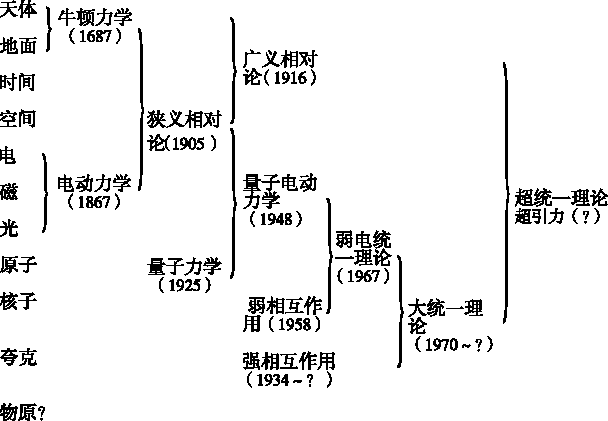
\includegraphics[width=0.98\linewidth]{figure/tab00.01} \\
    \bottomrule
    \zihao{6}* 括号中的数字表示相应的理论建立的年代;有问号的表示尚未完成。
  \end{tabular}
\end{tablex}
\clearpage\noindent 空观上是很不协调的。在前者中,各种匀速运动是平权的,但却
假定有绝对空间或绝对速度存在。相反,在后者中,有一个地位
特殊的速度,即光速,但却始终测不出这个特殊的速度是相对于
哪一个绝对空间而言的。爱因斯坦抛弃了绝对空间观念,使电磁
学、力学在新的时空观的基础上达到了协调和统一。

爱因斯坦还曾企图把引力和电磁力二者统一起来,但他的努
力没有成功。然而,他却找到了能与麦克斯韦电磁理论相协调的
引力理论——广义相对论。

作为引力理论的广义相对论和作为电磁理论的麦克斯韦理论
构成了我们今夭称为经典物理学的理论基础。

与经典物理相对的是量子论。量子力学最初是作为原子、分
子的统一的力学而发展起来的。这种新的力学统一地解释了原子、
分子的各种光谱现象,统一地解释了元素周期表,统一地解释了
各种不同分子的键合。

在将量子力学扩展到电磁场时,遇到了困难,这本质上是由
于电磁场是相对论性的。直到四十年代末,发展了所谓重整化方
法才巧妙地解决了上述的困难,使量子论与电磁理论能得以统一,
产生了量子电动力学。

到六十年代末,我们已经得到了如下的物理世界的图象。宇
宙中的所有物理对象可以分成两大类,一类称为“物质”,如夸
克、电子、$\mu$子等等,另一类称为“相互作用”,如引力、电磁力
等等。在目前的宇宙中,有四种基本的相互作用,按它们的强度
顺序排列是:核子参与的强相互作用,荷电粒子参与的电磁相互
作用,核子及电子、中微子参与的弱相互作用,以及任何粒子都
参与的引力相互作用。可以简单地说,宇宙间的一切运动和变化。
都可以统一为这四种“力”的作用。但是,追求统一的物理学,
似乎认为这种状况仍然不够统一。

1967年,温伯格和萨拉姆再次着眼于统一,先后提出了电磁
相互作用和弱相互作用的统一理论。随后的一系列实验证明他们
的统一理论是正确的。

这一新的成功,促使许多人去找寻把电磁作用、弱作用及强
作用都包含在内的统一理论,通常称为“大统一理论”。建立这
种理论的工作还没有完成,这是正在研究的领域。

如果大统一能够顺利完成,下一步的统一就是要把引力也统
一在内了。引力是物理学最早讨论的一种基本的力。但是,它与
其他力的统一最难,因为引力有一系列很特别的性质。例如这种
力只有引力却无斥力。就是这种特别性质之一。

企图把引力与其他力统一起来的工作,称为超统一的研究。
目前还没有得到有实际意义的结果。它是今天的物理学的一个前
沿。实现超统一的一个可能是用超引力理论,这种理论中的统一
有一个很有趣的特点,即它把物理学中传统的“物质”与“相互
作用”之间的界限也打破了。

总之,从牛顿力学开始,物理学就在寻找宇宙的统一,我们
希望找到控制着万事万物运动的极少的几个基点。只有从这个角
度我们才容易看清经典力学在整个物理学中的地位和作用,也才
能全面地了解学习经典力学对于学习整个物理学的意义和作用。
